% Please use the skeleton file you have received in the
% invitation-to-submit email, where your data are already
% filled in. Otherwise please make sure you insert your
% data according to the instructions in PoSauthmanual.pdf
\documentclass{PoS}
\usepackage{subcaption}

\title{Fast Calorimeter Simulation in LHCb}

\ShortTitle{Fast Calorimeter Simulation in LHCb}

\author{\speaker{Fedor Ratnikov}\thanks{on
    behalf of the LHCb collaboration}\\
        NRU Higher School of Economics, Moscow, Russia\\
        E-mail: \email{Fedor.Ratnikov@cern.ch}}

\author{Egor Zakharov\\
        Skolkovo Institute of Science and Technology, Moscow, Russia
%        E-mail: \email{...}
}

\abstract{
In HEP experiments, CPU resources required by MC simulations constantly grow and become a very large fraction of the required total computing power (greater than 75\%). At the same time, the pace of performance improvements from technology is slowing down. The only solution is a more efficient use of resources. LHC experiments seek options for simulating higher statistics events in a faster way. A key to the success of this strategy is the possibility of enabling fast simulation options in a common framework with minimal action by the final user. In this paper, we describe the solution to selectively exclude particles from being simulated by the Geant4 toolkit and to insert the corresponding hits generated in a faster way. The approach, integrated within the Geant4 toolkit, has been applied to the LHCb calorimeter, but it could also be used for other subdetectors. The hits generation can be carried out by any external tool, such as a static library of showers or more complex machine-learning techniques. Generative models, which are nowadays widely used for computer vision and image processing, are being studied as a candidate to accelerate the generation of showers in the calorimeter.  We present how both approaches can be applied to the LHCb calorimeter simulation, their advantages as well as their drawbacks.
}

\FullConference{The 39th International Conference on High Energy Physics (ICHEP2018)\\
        4-11 July, 2018\\
        Seoul, Korea}


\begin{document}

\section{Introduction}
During Run 2, the simulation of physics events at LHCb took about
80\% of the distributed computing resources, which were available to the
experiment \cite{LHCbCompUpgTDR}. The increase in the number of events, that will need to be simulated
in Run 3 to match the higher luminosity and trigger rate, will place an
extreme burden on the computing resources. To face this situation,
it is necessary to develop new ways to significantly increase the speed
of the simulation.

In a typical minimum bias event, calorimeter system takes about 55\% of the CPU time used by Geant4 \cite{geant4} to simulate particle transportation. 
Given this number, in the effort of developing a faster detector simulation, it is natural to start from the calorimeter.

A number of fast simulation options are available or are under development
in LHCb to complement the standard Geant4 based simulation. 
In this short paper, we consider two approaches to speed up a simulation of response in the electromagnetic calorimeter (ECAL): using pre-simulated
library of calorimeter responses, and generative model trained on
the pre-simulated sample.

The LHCb detector \cite{LHCb} is equipped with  ECAL, that employs a "shashlik" technology: alternating 4 mm thick
scintillator tiles and 2 mm thick lead plates are arranged perpendicular
to the beam pipe. The detector is not longitudinally segmented but
adopts a variable lateral segmentation,  because the hit density varies
by two orders of magnitude over the calorimeter surface. 
A segmentation into three different sections has been chosen for the ECAL: square cell sizes are of approximately 40, 60 and 120 mm in the inner, middle and outer regions, respectively.

%\begin{figure}[htb]
 % \begin{center}
  % 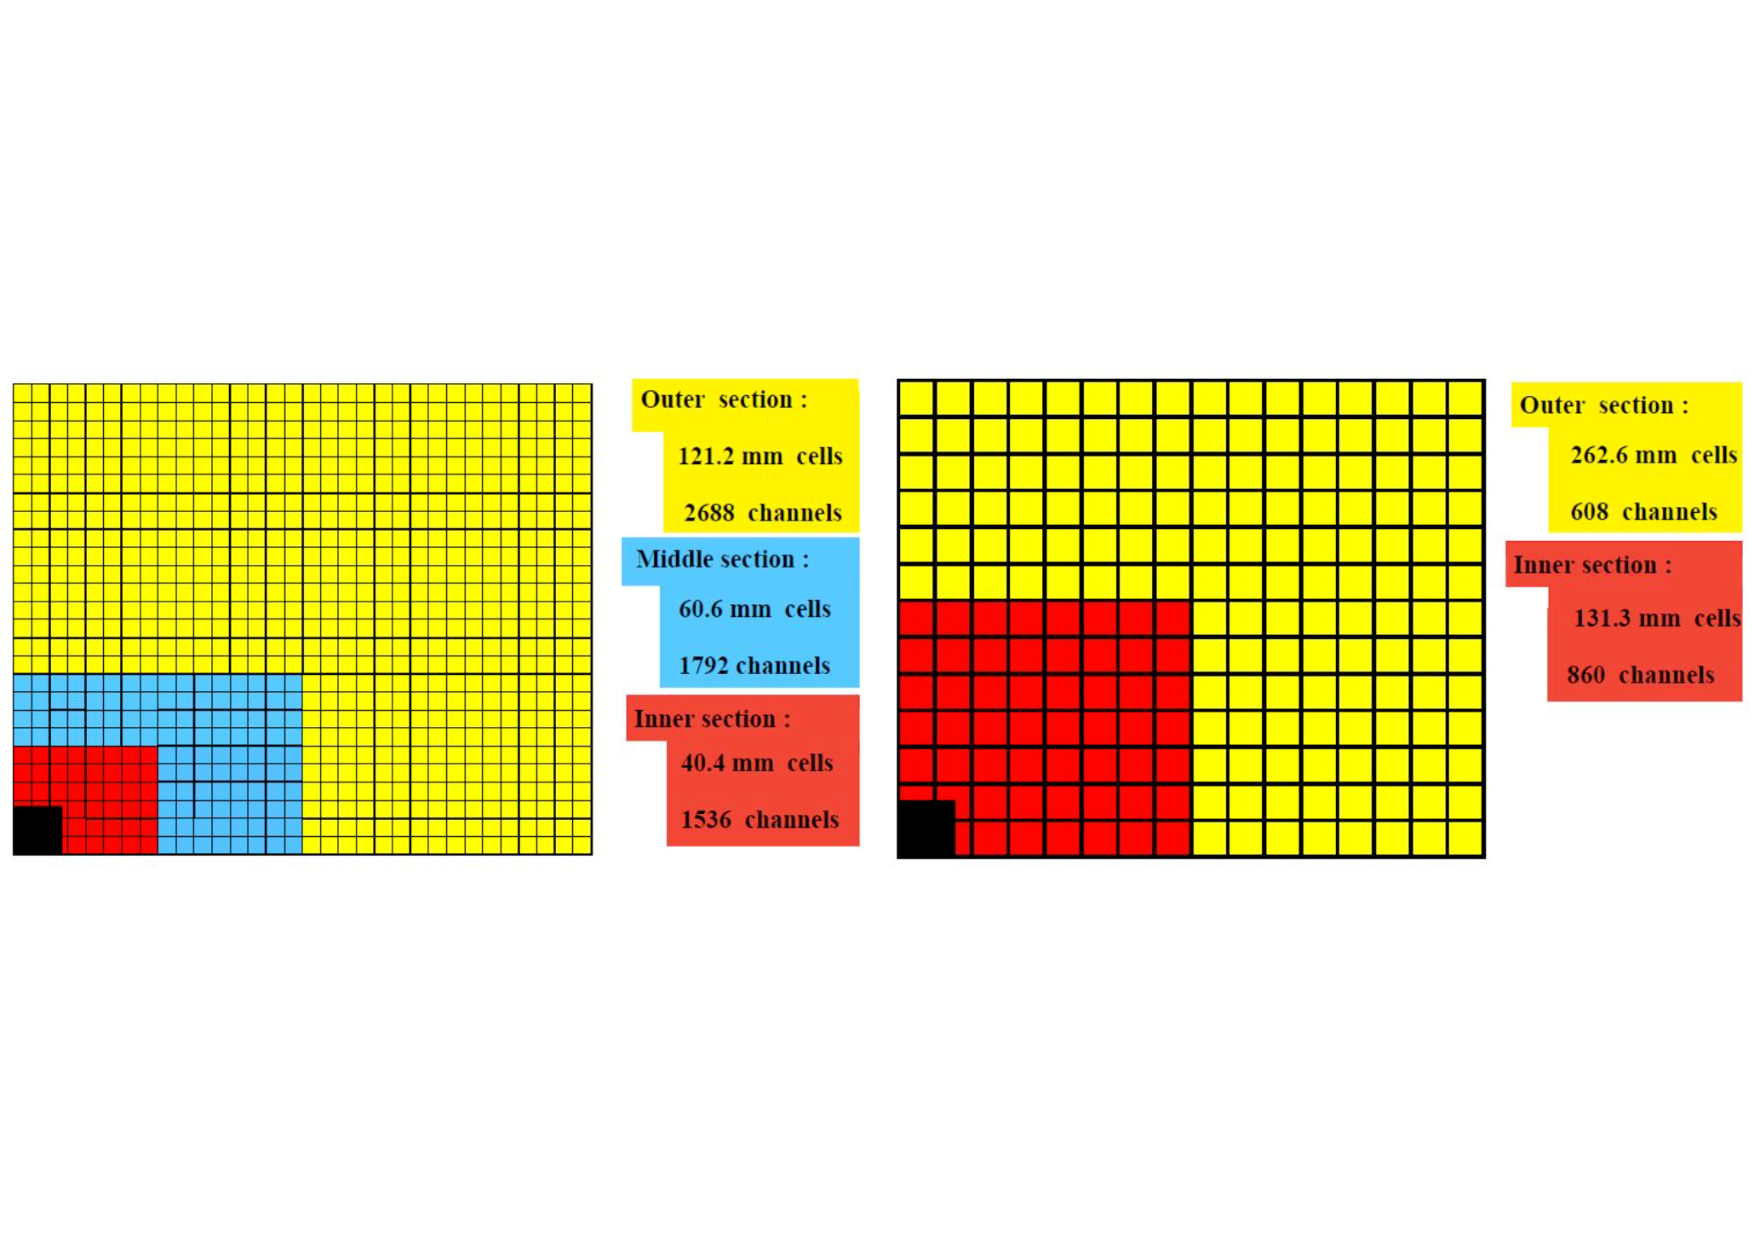
\includegraphics[width=1.0\textwidth]{figures/lhcbCalo.pdf}
  %  \caption{Lateral segmentation of the SPD/PRS and ECAL (left) and
   %   the HCAL (right). One quarter of the detector front face is
  %    shown. In the left figure the cell dimensions are given for the
 %     ECAL.\label{fig:lhcbCalo}}
 % \end{center}
%\end{figure}

\section{Library Approach \label{seq:LA}}
Details for this approach may be found elsewhere \cite{chepFastSim}.
To reduce the number of parameters in the produced response library, the
cell transverse area is divided into small subregions, or "points".
A library of points is built from simulated incident particles with
fixed values for particle position and azimuthal angle. Hence, for a
given particle species, only the binnings in energy and incidence angle remain. An example of point distribution in the ECAL, produced by an incident photon with energy O(1) GeV, is shown in Fig.~\ref{fig:pointProcessing}, top-left plot: each square of the grid represents the transverse area of an ECAL cell, and the colour scale indicates the deposited energy.
First, two or more points, belonging to the same cell area and with
associated energy below a given threshold, may be merged locally to
simplify the collection by reducing the number of points stored in
the library. This is exemplified in the top-right plot. Next, the points are shifted and rotated according to the position of
incidence and azimuthal angle of the particle with respect to the
values for which the library was built. This is a key aspect of the
point library. The collection of points represents a good model of the
shower projection in the transverse plane. Shift and
rotation of this collection give a good description of the shower produced by a translated and rotated incident particle. The rotation of the points
around the position of incidence of the particle is exemplified in
the bottom-left plot. Finally, the calorimeter hits are created by
summing the energies of those transformed points which fall into the
same cell area. This is shown in the bottom-right plot, where the
colour in the central region of the cell indicates the total deposited
energy.

\begin{figure}[htb]
  \begin{center}
   \begin{subfigure}[t]{0.4\textwidth}
    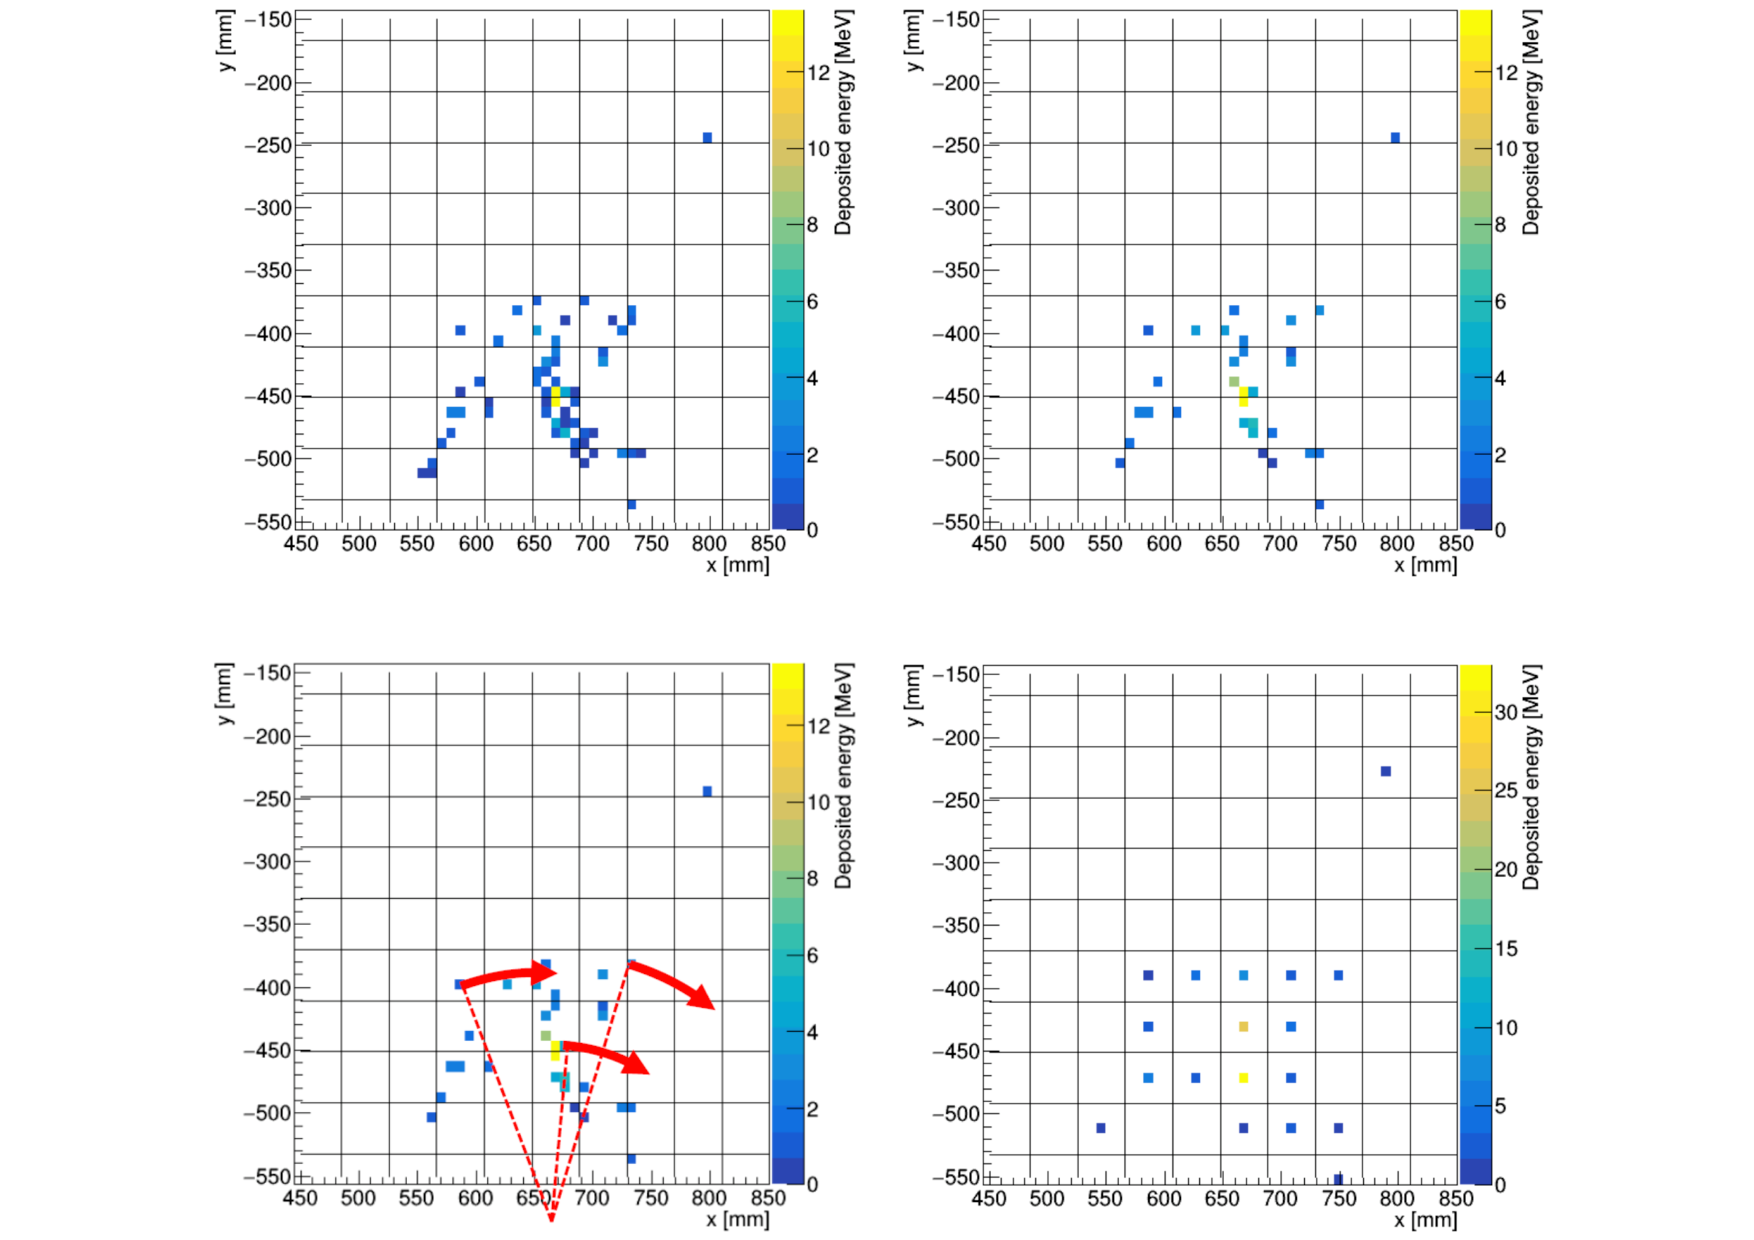
\includegraphics[width=1\textwidth]{figures/pointProcessing.pdf}
    \caption{Schematic illustration of the point library operating
      principle. More details are given in section
      \ref{seq:LA}.\label{fig:pointProcessing}}
  \end{subfigure}
  \hspace{0.04\textwidth}
   \begin{subfigure}[t]{0.52\textwidth}
    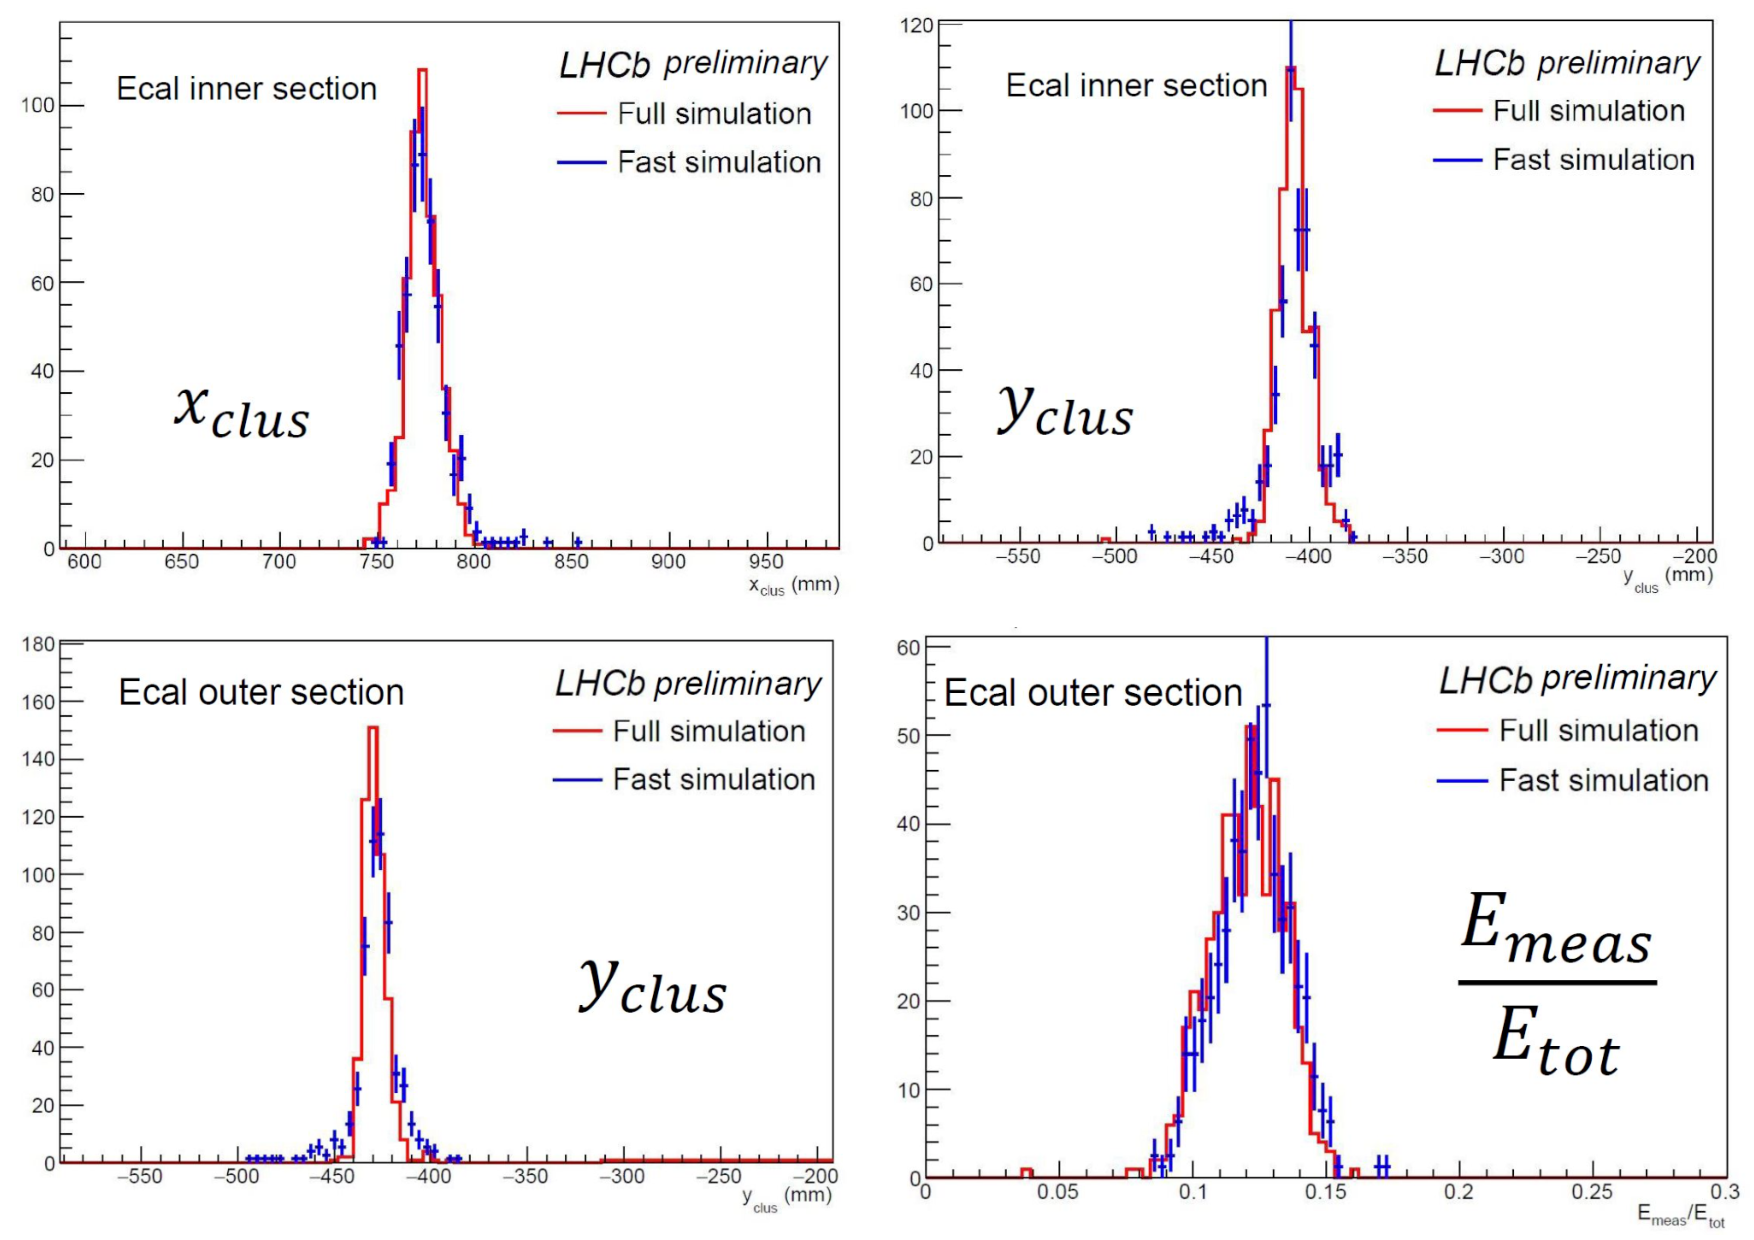
\includegraphics[width=1\textwidth]{figures/showerlibPerf.pdf}
    \caption{Comparison of photons simulated with Geant4 ("Full simulation") and with the point libraries ("Fast simulation") \label{fig:showerlibPerf}}
  \end{subfigure}
  \end{center}
\caption{Library approach.}
\end{figure}

The accuracy of the calorimeter simulation, based on point libraries,
has been tested through the comparison with the detailed simulation using
photons, generated at the calorimeter entrance with various energies
and angles of incidence. The coordinate of the hit cluster center is
calculated as a weighted average of coordinates of the cluster cells. 
Results are presented in Fig.~\ref{fig:showerlibPerf}.
The top plots compare the cluster position distributions in the simpler case,
where the entry point of the fully simulated photons coincides with
the entry point used to build a response in the library. Therefore, rotation alone is enough for the procedure described above.
The bottom plots correspond to a more complicated case, which compares distributions for cluster position and
measured energy, where the fully simulated photons are
generated in the outer sector. 
Therefore, the points had to be both rotated and shifted. However, the agreement does not worsen, that confirms the idea behind the point library.

\section {Generative Model Approach}
The idea of generic generative model approach  is to treat simulations as a black-box, and
to replace the traditional Monte Carlo simulation with a method based on
Generative Adversarial Networks \cite{gan}. 

We use Wasserstein GAN \cite{wgan}
with gradient penalty, which is considered to be a state-of-the-art technique
for the image production. The architecture of this Neural Network and details of training
the generative model are presented elsewhere \cite{chepGAN}.

After the generative model is built and trained,
we first compare the original clusters produced by full Geant4
simulation with the clusters generated by the trained model for the same
parameters of the incident particles: the same energy, the same
direction, and the same position on the calorimeter 
face. Corresponding images for the four arbitrary parameter sets are
presented in Fig.~\ref{fig:geant_vs_ours}. These images demonstrate very good visual similarity between simulated and generated clusters.

\begin{figure}
\captionsetup[subfigure]{justification=centering}
  \centering
  \begin{subfigure}{0.24\textwidth}
    \centering
    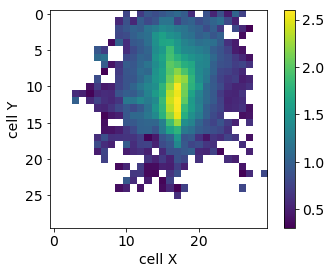
\includegraphics[width=1\textwidth]{figures/1_real.png}
  \end{subfigure}
  \begin{subfigure}{0.24\textwidth}
    \centering
    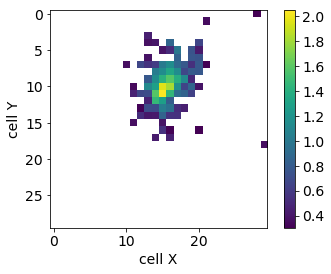
\includegraphics[width=1\textwidth]{figures/2_real.png}
  \end{subfigure}
    \begin{subfigure}{0.24\textwidth}
    \centering
    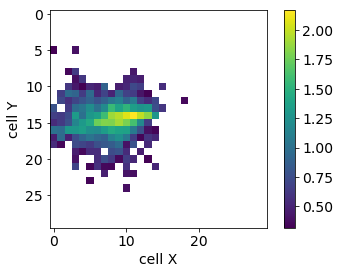
\includegraphics[width=1\textwidth]{figures/3_real.png}
  \end{subfigure}
  \begin{subfigure}{0.24\textwidth}
    \centering
    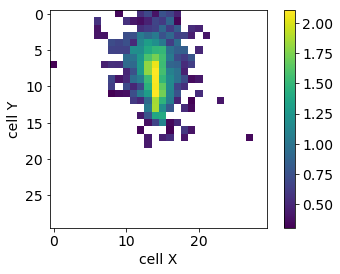
\includegraphics[width=1\textwidth]{figures/4_real.png}
  \end{subfigure}\\
   \begin{subfigure}{0.24\textwidth}
    \centering
    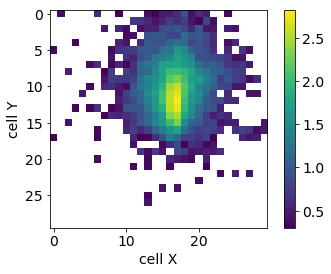
\includegraphics[width=1\textwidth]{figures/1_gen.png}
  \end{subfigure}
  \begin{subfigure}{0.24\textwidth}
    \centering
    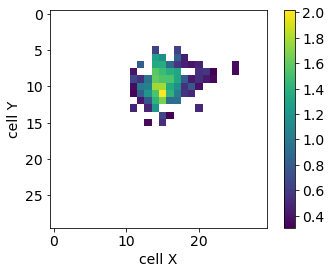
\includegraphics[width=1\textwidth]{figures/2_gen.png}
  \end{subfigure}
    \begin{subfigure}{0.24\textwidth}
    \centering
    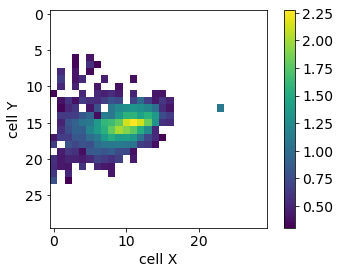
\includegraphics[width=1\textwidth]{figures/3_gen.png}
  \end{subfigure}
  \begin{subfigure}{0.24\textwidth}
    \centering
    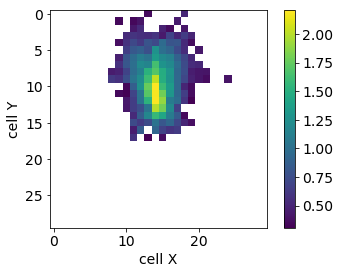
\includegraphics[width=1\textwidth]{figures/4_gen.png}
  \end{subfigure}
   \caption{Showers generated with GEANT4 (first row) and the showers,
    simulated with our model (second row) for three different sets of
    input parameters. Color represents $log_{10}(\frac{E}{MeV})$ for every cell.}
  \label{fig:geant_vs_ours}
\end{figure}

Then, we perform the quantitative evaluation of the proposed
simulation method. While generic evaluation methods for generative
models exist, we base our evaluation on
physics-driven similarity metrics. For this presentation, we selected
only a few cluster properties, which essentially drive the cluster properties used in the reconstruction of the calorimeter objects and following physics
analysis. If the initial particle direction is not perpendicular to the
calorimeter face, the produced cluster is elongated in that direction. 
Therefore, we separately consider cluster widths in the direction of the
initial particle and in the transverse direction. 
Spatial resolution, which is the distance between the center of mass of the
cluster and the initial track projection to the shower max depth, is
another important characteristic affecting physics properties of the
cluster.
 Cluster sparsity, which is the fraction of cells with energies above some threshold, reflects marginal low energy properties of the generated clusters. 
These characteristics are presented in Fig.~\ref{fig:ganquality}.

\begin{figure}[htb]
\begin{center}
 \begin{subfigure}[t]{0.3\textwidth}
      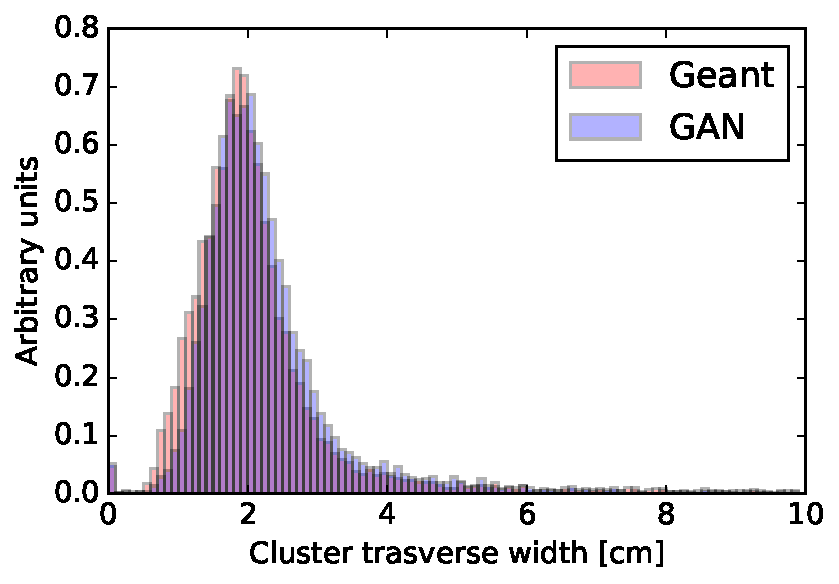
\includegraphics[width=1\textwidth]{figures/width_trans.pdf}
    \caption{The transverse width of real and generated clusters}
  \end{subfigure}\hspace{0.2\textwidth}
 \begin{subfigure}[t]{0.3\textwidth}
    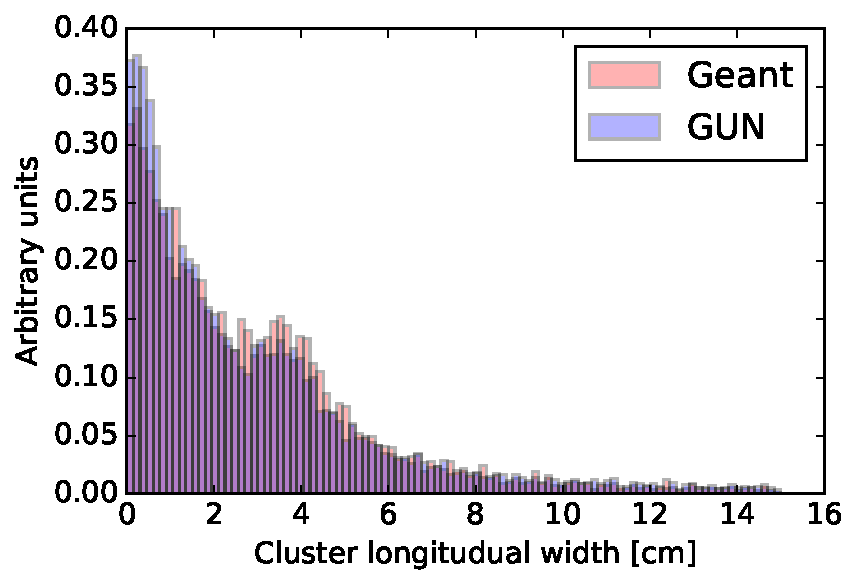
\includegraphics[width=1\textwidth]{figures/width_long.pdf}
    \caption{The longitudinal width of real and generated clusters}
  \end{subfigure}
\end{center}
\begin{center}
  \begin{subfigure}[t]{0.3\textwidth}
    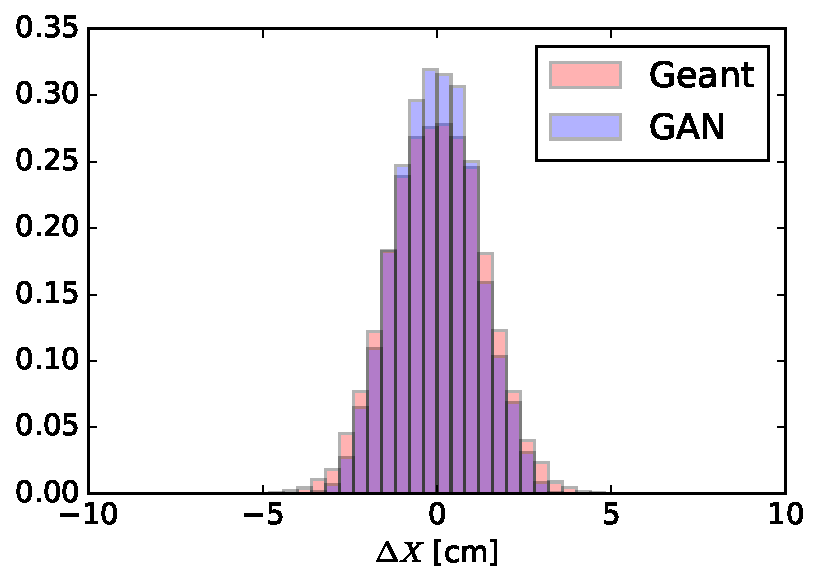
\includegraphics[width=1\textwidth]{figures/deltaX.pdf}
    \caption{$\Delta X$ between cluster center of mass and the true particle coordinate}
  \end{subfigure}\hspace{0.2\textwidth}
  \begin{subfigure}[t]{0.3\textwidth}
    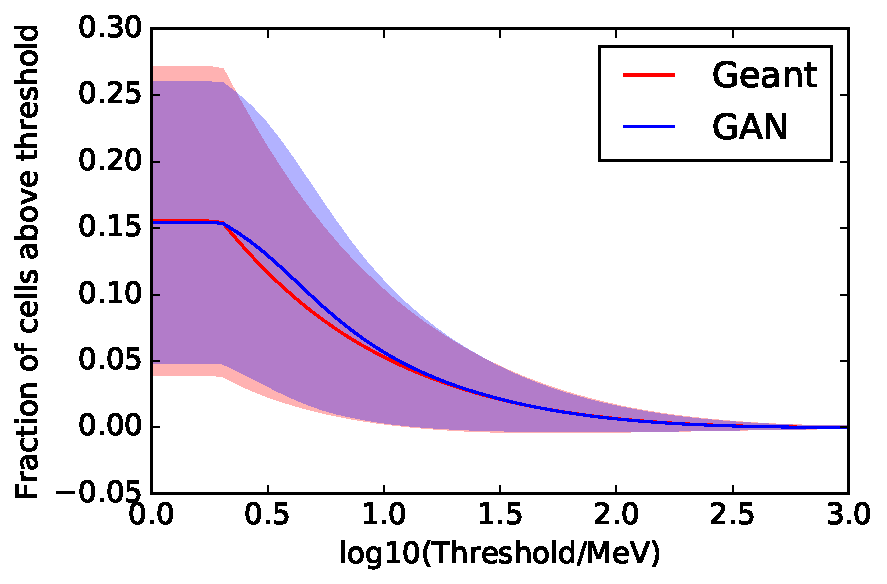
\includegraphics[width=1\textwidth]{figures/sparsity.pdf}
    \caption{The sparsity of real and generated clusters}
  \end{subfigure}
\end{center}
 \caption{Generated images quality evaluation including described
   physical characteristics.}\label{fig:ganquality}
\end{figure}


\section {Conclusions}
LHCb faces the current and future limitations of CPU resources with respect to the size of the necessary simulated samples.  This limitation leads to an ongoing effort to develop fast simulation
alternatives to the nominal detector simulation.  In the detailed simulation based on Geant4, more than 50\% of the CPU time is spent in the calorimeter system. We use different approaches to develop faster simulation of the calorimeter.
Both library and generative model approaches are encouraging in terms
of time gain and simulation accuracy.
The use of a point library, as opposed to a more standard cell hit library, significantly improves the output accuracy for the same size of the library.
We also confirm that Generative Adversarial Networks are a good
candidate for fast simulation of high granularity detectors, typically
considered for the next generation accelerators. 
We have successfully generated images of shower energy deposition with
a condition on the particle parameters, such as the momentum and the
coordinate, using modern generative deep neural network techniques.

%\bibliography{ichep18_ratnikov}

\begin{thebibliography}{99}
\bibitem{LHCbCompUpgTDR}LHCb collaboration, LHCb Upgrade Software and
  Computing Technical Design Report, CERN-LHCC-2018-007, LHCb-TDR-017.
\bibitem{geant4}S.Agostinelli et al.,(Geant4 Collaboration), Geant4:
  Asimulation toolkit,Nucl.Instrum. Methods Phys. Res., Sect. A 506, 250 (2003); J. Allison et al., (Geant4
  Collaboration), IEEE Trans. Nucl. Sci. 53, 270 (2006).
\bibitem{LHCb}LHCb collaboration, A. A. Alves Jr. et al., The LHCb detector at the LHC, JINST 3
(2008) S08005.
\bibitem{chepFastSim}M.Rama and G.Vitali (LHCb collaboration),
  Calorimeter fast simulation based on hit libraries in the LHCb Gauss
  framework, proceedings of CHEP2018 conference, to be published in the
  EPJ Web of Conferences.
\bibitem{gan}I. Goodfellow, J. Pouget-Abadie, M. Mirza, B. Xu, D. Warde-Farley, S. Ozair,
A. Courville, Y. Bengio, Generative adversarial nets, in Advances in neural information
processing systems (2014), pp. 2672-2680.
\bibitem{wgan}T.C. Wang, M.Y. Liu, J.Y. Zhu, G. Liu, A. Tao, J. Kautz, B. Catanzaro, arXiv preprint
arXiv:1808.06601 (2018).
\bibitem{chepGAN}V.Chekalina et al., Generative Models for Fast Calorimeter Simulation: LHCb case, proceedings of CHEP2018 conference, to be published in the
  EPJ Web of Conferences.
\end{thebibliography}

\end{document}

